\documentclass{article}
\usepackage[utf8]{inputenc}
\usepackage[spanish]{babel}
\usepackage{listings}
\usepackage{graphicx}
\graphicspath{ {images/} }
\usepackage{cite}

\begin{document}

\begin{titlepage}
    \begin{center}
        \vspace*{1cm}
            
        \Huge
        \textbf{Cambio de posicion de un objeto}
            
        \vspace{0.5cm}
        \LARGE
        Subtítulo
            
        \vspace{1.5cm}
            
        \textbf{Karen López Aljure}
            
        \vfill
            
        \vspace{0.8cm}
            
        \Large
        Despartamento de Ingeniería Electrónica y Telecomunicaciones\\
        Universidad de Antioquia\\
        Medellín\\
        Marzo de 2021
            
    \end{center}
\end{titlepage}

\tableofcontents
\newpage
\section{Sección introductoria}\label{intro}
El siguiente trabajo consiste en describir de forma detallada como llevar unos objetos de una posición A a una posición B,para lo cual se adjuntará un video con la demostracón de que el objetivo fue logrado.

\section{Sección de contenido} \label{contenido}

\subsection{Instrucciones}
1.	leer atentamente las siguientes instrucciones.

2.	tener materiales (hoja de papel lisa, dos tarjetas preferiblemente de la misma densidad).


3.	colocar la hoja de papel en la superficie plana(mesa).

4.	coger las dos tarjetas con una mano (puede ser izquierda o derecha).


5.	con la mano que escoja, agarrar la hoja de papel y levantarla.

6.	con la mano que tenga libre colocar debajo de la hoja de papel las dos tarjetas.


7.	soltar las tarjetas y dejarlas ahí.

8.	levantar la hoja de papel y sacar las tarjetas usando solo una mano y sostenerlas (puede ser la mano izquierda o derecha).


9.	con esa misma mano colocar frente a frente las dos tarjetas de forma vertical quedando al mismo nivel y apoyarlas encima de la hoja de papel.

10.	con el dedo pulgar y el dedo índice inicialmente ir separando las tarjetas por la parte inferior de donde inicialmente se sostienen, tratando de formar un Angulo agudo (tiene menos de 90 grados ), si ve la necesidad de ayudarse con los dedos medio, anular y meñique puede utilizarlos.


11.	 cuando ya se logre un equilibrio entre las dos tarjetas (que estas se puedan sostener apoyándose entre ellas mismas formando una pirámide) ir despegando los dedos uno a uno cuidadosamente hasta soltar las tarjetas completamente. 

12.	si se logra observar las dos tarjetas apoyándose una sobre la otra formando la pirámide sin ningún apoyo extra, el objetivo lo logro con exito. 


13.	si no lo logra volverlo a intentar. 



\subsection{Recomendaciones}
%
para realizar esta actividad se recomienda leer previamente la instrucciones dadas en este documento , adémas de tener una buena concentración al  momento de intentar hacer la actividad.


\section{Inclusión de imágenes} \label{imagenes}

En la Figura se muestra un ejemplo de como debe de quedar terminada la actividad.

\begin{figure}[h]
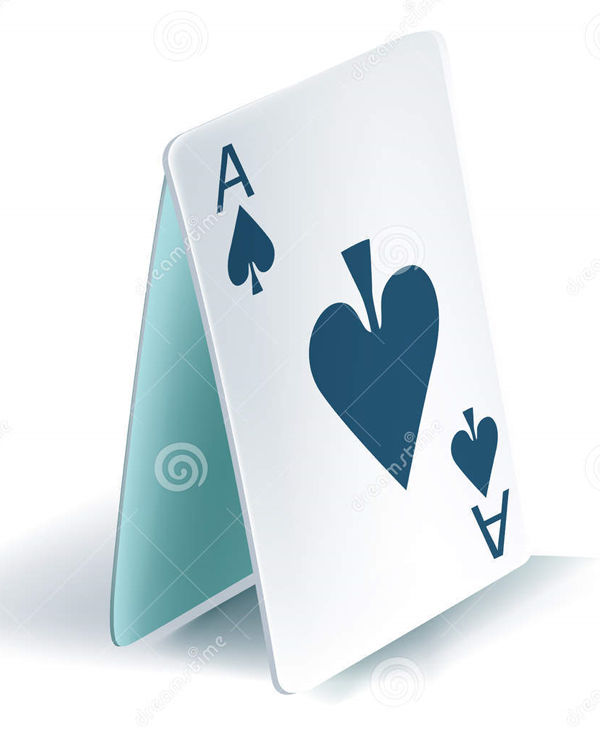
\includegraphics[width=4cm]{piramide.png}
\centering
\caption{piramide}
\label{fir:piramide}
\end{figure}


\label{imagenes}

\end{document}
